\documentclass[border=0mm]{standalone}
\usepackage{pgfplots}
\usepgfplotslibrary{groupplots}
\pgfplotsset{compat=1.17}
\usepackage{xcolor}
\usepackage{xstring}
\usepackage{ upgreek }
\usepackage{amsmath}
\definecolor{blue}{rgb}{0,0.4470,0.7410}




\pgfplotsset{
compat=1.11,
legend image code/.code={
\draw[mark repeat=2,mark phase=2]
plot coordinates {
(0cm,0cm)
(0.15cm,0cm)        %% default is (0.3cm,0cm)
(0.3cm,0cm)         %% default is (0.6cm,0cm)
};%
}
}%
\definecolor{lightblue}{RGB}{86,192,150}  % Define light blue color
\pgfdeclarelayer{background layer}%
\pgfdeclarelayer{foreground layer}%
\pgfsetlayers{background layer,main,foreground layer}%
\begin{document}
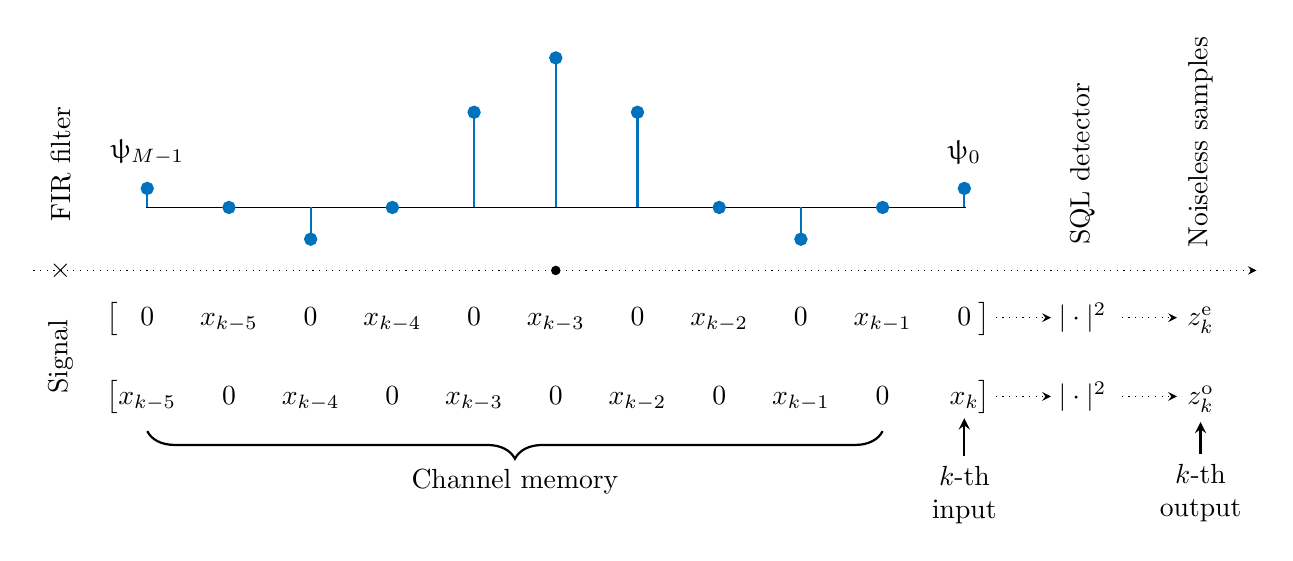
\begin{tikzpicture}[
declare function={
	sinc(\x) = (\x == 0) * 1+
			(\x!=0) * sin(pi*deg(\x))/(pi*\x) ;
},
>=stealth
]
\begin{axis}[
  width = 12cm,
  height = 5cm,
  axis x line*=middle,  % Show only the x-axis
  axis y line=none,    % Hide the y-axis
  xmin=-2.51, xmax=2.51,
  ymin=-0.5, ymax=1.3,  % Set ymax to 2
  xtick=\empty,
  every tick label/.append style={scale=0.7},
  xlabel style={
    right,
  },
  legend style={draw=none,nodes={scale=0.4, transform shape}}
]%

\addplot [thick,ycomb, domain=-2.5:2.5, samples=11, blue, mark=*] {sinc(x)};

\coordinate (p0) at (axis cs: -2.5,0);
\coordinate (p1) at (axis cs: -2,0);
\coordinate (p2) at (axis cs: -1.5,0);
\coordinate (p3) at (axis cs: -1,0);
\coordinate (p4) at (axis cs: -0.5,0);
\coordinate (p5) at (axis cs: 0,0);
\coordinate (p6) at (axis cs: 0.5,0);
\coordinate (p7) at (axis cs: 1,0);
\coordinate (p8) at (axis cs: 1.5,0);
\coordinate (p9) at (axis cs: 2,0);
\coordinate (p10) at (axis cs: 2.5,0);


\end{axis}%

\draw [fill]  ($(p5)+(0,-.8)$) circle (1.5pt) node (point) {};

\node [anchor=base] at ($(p10)+(0.25,-1.5)$) {$\bigr]$};
\node [anchor=base] at ($(p10)+(0,-1.5)$) {$0$};
\node [anchor=base] at ($(p9)+(0,-1.5)$) {$x_{k-1}$};
\node [anchor=base] at ($(p8)+(0,-1.5)$) {$0$};
\node [anchor=base] at ($(p7)+(0,-1.5)$) {$x_{k-2}$};
\node [anchor=base] at ($(p6)+(0,-1.5)$) {$0$};
\node [anchor=base] at ($(p5)+(0,-1.5)$) {$x_{k-3}$};
\node [anchor=base] at ($(p4)+(0,-1.5)$) {$0$};
\node [anchor=base] at ($(p3)+(0,-1.5)$) {$x_{k-4}$};
\node [anchor=base] at ($(p2)+(0,-1.5)$) {$0$};
\node [anchor=base] at ($(p1)+(0,-1.5)$) {$x_{k-5}$};
\node [anchor=base] at ($(p0)+(0,-1.5)$) {$0$};
\node [anchor=base] at ($(p0)+(-0.45,-1.5)$) {$\bigl[$};

\node [anchor=base] (xd) at ($(p10)+(0.25,-2.5)$) {$\bigr]$};
\node [anchor=base] (present_samp) at ($(p10)+(0,-2.5)$) {$x_{k}$};
\node [anchor=base] at ($(p9)+(0,-2.5)$) {$0$};
\node [anchor=base] at ($(p8)+(0,-2.5)$) {$x_{k-1}$};
\node [anchor=base] at ($(p7)+(0,-2.5)$) {$0$};
\node [anchor=base] at ($(p6)+(0,-2.5)$) {$x_{k-2}$};
\node [anchor=base] at ($(p5)+(0,-2.5)$) {$0$};
\node [anchor=base] at ($(p4)+(0,-2.5)$) {$x_{k-3}$};
\node [anchor=base] at ($(p3)+(0,-2.5)$) {$0$};
\node [anchor=base] at ($(p2)+(0,-2.5)$) {$x_{k-4}$};
\node [anchor=base] at ($(p1)+(0,-2.5)$) {$0$};
\node [anchor=base] at ($(p0)+(0,-2.5)$) {$x_{k-5}$};
\node [anchor=base] at ($(p0)+(-0.45,-2.5)$) {$\bigl[$};

\node [] at ($(p10)+(0,0.7)$) {$\uppsi_{0}$};
\node [] at ($(p0)+(0,0.7)$) {$\uppsi_{M-1}$};

\draw [<-,thick] (present_samp) -- +(0,-0.7) node[below, text width=1.4cm,align=center] {$k$-th input};
\draw [thick,decorate,decoration={brace,amplitude=10pt,mirror,raise=4pt},yshift=0pt]
($(p0)+(0,-2.7)$) -- node [below,yshift=-0.5cm] {Channel memory}($(p9)+(0,-2.7)$);

\draw [black, dotted] (point) --+ (-6.29,0) node (left_coord){} --+ (-6.7,0);
\draw [->,black, dotted] (point) --+ (6.29,0) node (right_coord){} --+ (8.9,0);

\node [rotate = 90,anchor=west] at ($(left_coord)+(0,0.5)$) {FIR filter};
\node [rotate = 90] at (left_coord) {$\times$};
\node [rotate = 90,anchor=east] at ($(left_coord)+(0,-0.5)$) {Signal};

\node [anchor=base] (sqle) at ($(p10)+(1.5,-1.5)$) {$|\cdot|^2$};
\node [anchor=base] (even) at ($(p10)+(3,-1.5)$) {$z_k^{\text{e}}$};

\node [anchor=base] (sqlo) at ($(p10)+(1.5,-2.5)$) {$|\cdot|^2$};
\node [anchor=base] (odd) at ($(p10)+(3,-2.5)$) {$z_k^{\text{o}}$};

\draw [dotted,->] ($(p10)+(.4,-2.4)$) -- ($(p10)+(1.1,-2.4)$);
\draw [dotted,->] ($(p10)+(2,-2.4)$) -- ($(p10)+(2.7,-2.4)$);

\draw [dotted,->] ($(p10)+(.4,-1.4)$) -- ($(p10)+(1.1,-1.4)$);
\draw [dotted,->] ($(p10)+(2,-1.4)$) -- ($(p10)+(2.7,-1.4)$);

\draw [<-,thick] (odd) -- +(0,-0.7) node[below, text width=1.4cm,align=center] {$k$-th output};

\node [rotate=90, anchor=west] at ($(sqle)+(0,0.8)$) {SQL detector};
\node [rotate=90, anchor=west] at ($(even)+(0,0.8)$) {Noiseless samples};

\end{tikzpicture}%
\end{document}
























